% ==========================================
% CHAPITRE 1
% ==========================================
\chapter{Contexte Général}

\vspace{2.5cm}

\noindent \textbf{\Large Plan}
\vspace{0.8cm}

\begin{enumerate}[label=\textbf{\arabic*}, leftmargin=1.5cm, labelsep=0.8cm]
    \item \textbf{Organisme d'accueil} \dotfill \pageref{sec:organisme}
    \item \textbf{Présentation du projet} \dotfill \pageref{sec:presentation}
    \item \textbf{La démarche adoptée} \dotfill \pageref{sec:demarche}
    \item \textbf{Langage de Modélisation UML} \dotfill \pageref{sec:uml}
\end{enumerate}

\vfill
\newpage

\section*{Introduction}
Dans ce chapitre, nous présenterons tout d'abord l'entreprise d'accueil dans laquelle nous avons effectué notre stage de fin d'études. Nous procéderons ensuite à une analyse de l'existant sur le marché, afin d'identifier les pratiques et solutions actuellement utilisées. Enfin, nous détaillerons la démarche méthodologique adoptée pour la conception et le développement de notre projet.

\section{Organisme d'accueil : Grow Up Technologies}\label{sec:organisme}

Le présent projet de fin d'études a été réalisé au sein de \textbf{Grow Up Technologies}, une entreprise tunisienne innovante spécialisée dans le développement de solutions logicielles sur mesure. En se positionnant comme un partenaire technologique agile, l'entreprise se distingue par l'intégration systématique de l'Intelligence Artificielle (IA) au cœur de ses processus, accompagnant ainsi les PME et les grandes organisations dans leur transformation numérique à travers la Tunisie, l'Europe (France, Belgique, Suisse) et l'Amérique du Nord (Québec).

\vspace{0.3cm}
L'expertise de l'entreprise s'articule autour de quatre axes majeurs :
\begin{itemize}[label=\textbullet, leftmargin=1.5cm]
    \item \textbf{Ingénierie logicielle Web et Mobile :} Conception d'applications personnalisées, performantes et évolutives, répondant aux exigences spécifiques de chaque secteur d'activité.
    \item \textbf{Automatisation des processus :} Mise en œuvre de solutions intelligentes visant à optimiser la productivité opérationnelle en réduisant les tâches manuelles chronophages.
    \item \textbf{Chatbots et agents IA :} Développement de systèmes conversationnels avancés pour fluidifier les interactions utilisateurs et moderniser le support client.
    \item \textbf{Solutions d'IA générative :}~\cite{llm_survey} Exploitation de modèles de pointe pour la production de contenus et l'aide à la décision dans divers contextes professionnels.
\end{itemize}
\vspace{0.5cm}

\noindent La vision de Grow Up Technologies repose sur la fusion entre l'ingénierie logicielle classique et les technologies de rupture. Cette synergie permet de transformer des problématiques complexes en leviers de croissance concrets, tout en démocratisant l'accès aux outils d'intelligence artificielle pour l'ensemble de ses partenaires francophones.

\begin{figure}[h!]
    \centering
    
\includegraphics[width=0.6\textwidth]{logo grow up .png}
    \caption{Logo de Grow Up Technologies}
    \label{fig:logo_growup}
\end{figure}

\section{Présentation du Projet}\label{sec:presentation}
PaieZone RH est un module métier développé dans le cadre de la plateforme SaaS ComptaZone, une solution intégrée destinée aux experts-comptables et aux cabinets comptables tunisiens. ComptaZone a pour ambition de centraliser l'ensemble des outils de gestion utilisés par les professionnels du chiffre --- comptabilité générale, facturation, déclarations fiscales, gestion RH et paie --- au sein d'une seule plateforme en ligne, accessible depuis n'importe quel appareil et en tout lieu.

\subsection{Analyse de l'Existant}
Il est nécessaire, avant la réalisation d'un tel projet, d'étudier les projets similaires dans le but de profiter de leurs avantages et de dégager leurs inconvénients.

\subsection{État de l'art : Le marché de la gestion RH et paie en Tunisie}

L'analyse du marché tunisien révèle une coexistence entre méthodes traditionnelles et solutions numériques émergentes. Ces approches peuvent être classifiées en trois catégories principales selon leur maturité technologique et leur accessibilité.

\vspace{0.4cm}

\noindent \textbf{1. Les feuilles de calcul (Approche manuelle)} \\
Excel reste la solution la plus répandue dans les PME tunisiennes pour le calcul de la paie.
Son utilisation est souvent le résultat d'un manque de budget ou d'une méconnaissance des
outils spécialisés. Le comptable crée manuellement des formules de calcul CNSS et IRPP,
maintient des tableaux de suivi des congés et génère des bulletins en formatant manuellement
des cellules.

\vspace{0.3cm}

\noindent \textbf{2. Les logiciels Desktop (Solutions locales spécialisées)} \\
Plusieurs logiciels de gestion de paie desktop sont disponibles sur le marché tunisien. Parmi
les plus utilisés, on retrouve des solutions comme les logiciels proposés par Megasoft ERP,
PGPRO Tunisie, DSPAYE et d'autres éditeurs locaux. Ces solutions offrent des
fonctionnalités de calcul de bulletin de paie, de gestion des cotisations CNSS, de gestion des
congés et d'édition de déclarations. Elles sont généralement installées sur un poste de travail
et fonctionnent avec une base de données locale (SQL Server, Access).

\vspace{0.3cm}

\noindent \textbf{3. Les solutions Cloud et Plateformes (SaaS)} \\
Paie-tunisie.com est décrit comme le premier site tunisien dédié à la gestion en ligne de la
paie et aux informations juridico-sociales. Lancé par des experts comptables et des
compétences en ingénierie informatique, il permet aux PME, professions libérales et
structures moyennes de gérer en ligne l'édition de fiches de paie. La plateforme propose un
simulateur de paie intégrant le barème d'imposition de la Loi de Finances 2026~\cite{loifinance},
une solution d'essai gratuite d'un mois, et des solutions payantes avec abonnement mensuel.
Elle inclut également une base documentaire sur les réglementations (code du travail,
conventions collectives, CNSS~\cite{cnss_reg}, lois de finances).

\begin{figure}[h!]
    \centering
    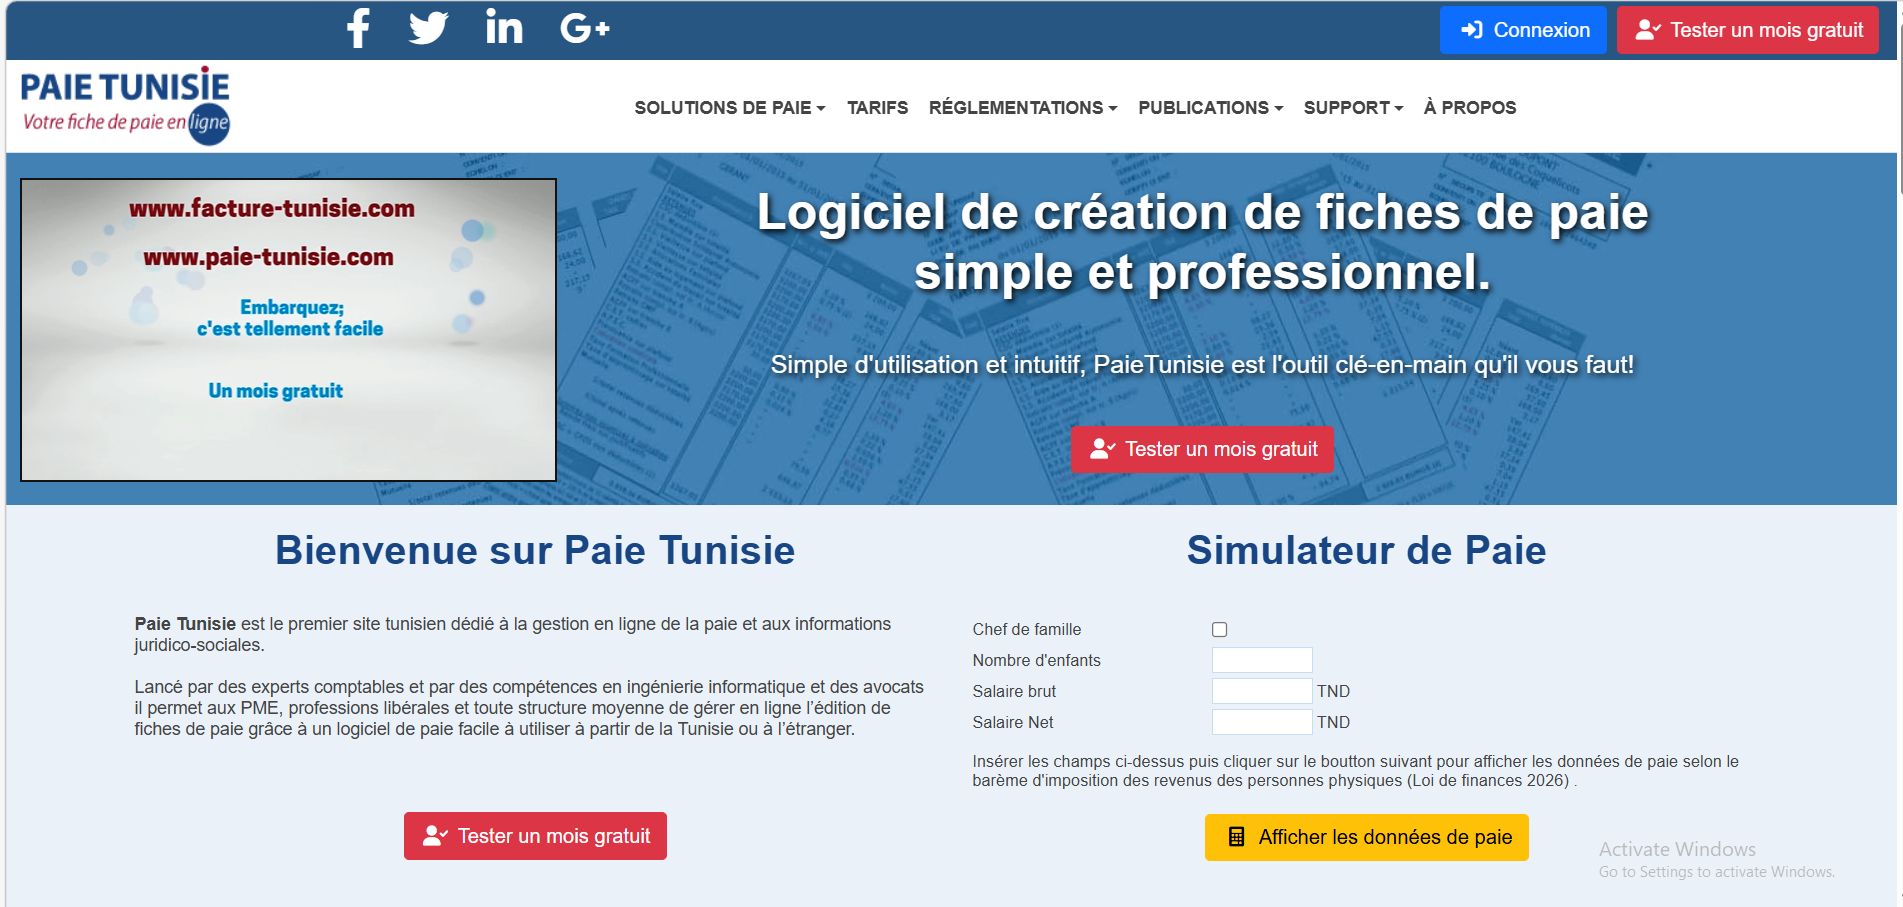
\includegraphics[width=0.9\textwidth]{paie tunisie.png}
    \caption{Paie tunisie}
\end{figure}

\subsection{Comparaison avec l'existant}
Le tableau~\ref{tab:comparaison_finale} présente une étude comparative détaillée des principales solutions de gestion RH et paie disponibles sur le marché tunisien, en les confrontant à la solution proposée PaieZone RH.

\renewcommand{\arraystretch}{2.2}
\begin{longtable}{|>{\raggedright\arraybackslash\bfseries}p{3.5cm}|>{\centering\arraybackslash}p{2.3cm}|>{\centering\arraybackslash}p{2.3cm}|>{\centering\arraybackslash}p{2.8cm}|>{\centering\arraybackslash}p{2.3cm}|}

\hline
\rowcolor[HTML]{EFEFEF}
Critères de comparaison & Excel & Logiciel Desktop & paie-tunisie.com & PaieZone RH \\ \hline
\endfirsthead

\hline
\rowcolor[HTML]{EFEFEF}
Critères de comparaison & Excel & Logiciel Desktop & paie-tunisie.com & PaieZone RH \\ \hline
\endhead

\hline
\endfoot

\caption{Étude comparative détaillée des solutions de gestion RH et paie}
\label{tab:comparaison_finale}
\endlastfoot

Accessibilité & Local uniquement & Local uniquement & Web navigateur & Web et API \\ \hline
Multi-tenant (Cabinet) & Non & Non & Non & Oui (Schéma dédié) \\ \hline
Calcul CNSS / IRPP & Manuel (formules) & Automatique & Automatique & Automatique + versionné \\ \hline
Mise à jour (Loi 2026) & Manuelle & Mise à jour éditeur & Partielle & Automatique centralisée \\ \hline
Gestion des congés & Tableau manuel & Basique & Basique & Workflow multi-niveaux \\ \hline
Pointage et Temps & Non & Partiel & Non & Complet (Badge, Import) \\ \hline
GED / Documents RH & Non & Non & Non & Oui (Archivage + Expiry) \\ \hline
Intégration comptable & Non & Partielle & Non & Auto (Plan comptable) \\ \hline
Déclarations officielles & Non & Oui & CNSS uniquement & CNSS, CAVIS, IRPP \\ \hline
Chatbot IA / RAG & Non & Non & Non & \textbf{Oui (Multi-canal)} \\ \hline
Authentification 2FA & Non & Non & Non & Oui (TOTP) \\ \hline
Journal d'audit & Non & Non & Non & Complet (Toutes actions) \\ \hline
API REST documentée & Non & Non & Non & Oui (Swagger) \\ \hline

\end{longtable}
\renewcommand{\arraystretch}{1.0}

L'analyse des solutions de gestion RH et paie disponibles sur le marché tunisien met en évidence plusieurs lacunes technologiques et fonctionnelles qui freinent l'efficacité opérationnelle des entreprises.

\begin{itemize}[label=\textbullet, leftmargin=1.5cm]
    \item \textbf{Absence d'IA et d'automatisation intelligente :}
    Aucune solution locale n'intègre actuellement d'intelligence artificielle~\cite{llm_survey}. Les interactions restent purement manuelles : l'employé doit solliciter directement le service RH pour chaque besoin (attestations, bulletins, congés). L'absence de chatbots ou d'agents conversationnels s'exprimant en langage naturel s'accompagne d'une surcharge de travail pour les gestionnaires et d'une expérience utilisateur limitée~\cite{chatbot_hr}.

    \item \textbf{Déficit de mobilité et de flexibilité (Cloud/SaaS) :}
    La prédominance des logiciels desktop restreint l'accès aux données à un poste de travail physique unique~\cite{saas}. Cette architecture interdit le travail à distance pour le comptable, la validation mobile pour le manager et la consultation en libre-service pour l'employé. De plus, le manque d'architecture multi-tenant~\cite{multitenant} empêche une gestion unifiée de plusieurs portefeuilles clients pour les cabinets d'expertise.

    \item \textbf{Lourdeur des processus administratifs :}
    La gestion des dossiers (contrats, documents administratifs, pointages) repose encore sur de nombreuses saisies répétitives. Les solutions actuelles manquent de \textit{workflows} de validation multi-niveaux automatisés (Employé $\rightarrow$ Manager $\rightarrow$ RH) et de systèmes de notifications intelligentes pour les événements critiques, tels que l'expiration des contrats CDD ou les reliquats de congés.

    \item \textbf{Complexité des mises à jour réglementaires :}
    L'évolution annuelle de la législation (notamment la \textbf{Loi de Finances 2026}~\cite{loifinance}) impose une veille constante. Sur les logiciels classiques, la mise à jour des barèmes IRPP, des taux CNSS~\cite{cnss_reg} ou du SMIG nécessite une intervention manuelle ou une réinstallation logicielle. Ce processus rigide augmente le risque d'erreurs de calcul, pouvant entraîner des bulletins non conformes et des sanctions fiscales.
\end{itemize}

\vspace{0.3cm}

\noindent Ces insuffisances justifient le besoin d'une solution moderne, centrée sur l'automatisation par l'IA et l'accessibilité SaaS~\cite{saas}, afin de répondre aux exigences de conformité et de productivité des organisations tunisiennes.

\subsection{Solution Proposée : La Plateforme PaieZone RH}\label{sec:solution}

Pour répondre aux lacunes du marché, nous proposons le développement de \textbf{PaieZone RH}, une solution SaaS multi-tenant~\cite{multitenant} nativement conçue pour moderniser la gestion sociale en Tunisie.

\subsubsection{Description et Périmètre Fonctionnel}
L'application repose sur une architecture moderne de microservices logiques. Elle centralise l'intégralité du cycle RH à travers les axes suivants :
\begingroup
\begin{itemize}[label=\textbullet, leftmargin=1.5cm]
    \item \textbf{Gestion administrative et contractuelle :} Suivi exhaustif des dossiers employés et pilotage des contrats spécifiques au droit tunisien~\cite{cdt} (CDI, CDD, CIVP, KARAMA, Stage).
    \item \textbf{Moteur de paie conforme :} Calcul automatisé intégrant les règles fiscales et sociales de la Loi de Finances 2026~\cite{loifinance} (CNSS~\cite{cnss_reg}, CAVIS, IRPP).
    \item \textbf{Pilotage des temps et activités :} Gestion dématérialisée des congés avec workflows de validation et suivi automatisé du pointage.
    \item \textbf{Déclarations et comptabilité :} Génération automatique des documents légaux et intégration fluide des écritures comptables.
    \item \textbf{Innovation IA :} Intégration d'un Chatbot RH intelligent~\cite{chatbot_hr} basé sur une architecture \textbf{RAG} (Retrieval Augmented Generation)~\cite{rag_paper}, permettant une interaction en langage naturel avec la base documentaire de l'entreprise.
\end{itemize}
\endgroup
\subsubsection{Valeur ajoutée du modèle SaaS et de l'IA}
L'adoption d'une architecture Cloud~\cite{saas} couplée à l'intelligence artificielle offre des avantages stratégiques déterminants :
\begingroup
\begin{itemize}[label=\textbullet, leftmargin=1.5cm]
    \item \textbf{Accessibilité et Mobilité :} Disponibilité universelle sur tous les terminaux, éliminant les contraintes d'installation locale et favorisant le travail collaboratif.
    \item \textbf{Efficience Multi-tenant :} Capacité pour un cabinet comptable ou une direction RH de piloter plusieurs entités (tenants)~\cite{multitenant} via une interface unique, sécurisée et isolée au niveau de la base de données.
    \item \textbf{Agilité Réglementaire :} Déploiement centralisé et instantané des mises à jour fiscales~\cite{loifinance}, garantissant une conformité permanente sans intervention manuelle des utilisateurs.
    \item \textbf{Self-service Employé par l'IA :}
    L'intégration du Chatbot RH IA~\cite{chatbot_hr} apporte une dimension innovante au self-service employé en garantissant une disponibilité continue 24h/24. Cette réactivité permet aux salariés d'obtenir un support immédiat pour leurs requêtes courantes sans solliciter directement les gestionnaires RH, optimisant ainsi le temps de chacun. Au-delà de la simple assistance, le chatbot est capable d'effectuer des automatisations directes, telles que la soumission d'une demande de congé ou la récupération instantanée d'un bulletin de paie. Enfin, grâce au système RAG~\cite{rag_paper}, l'outil fait preuve d'une véritable intelligence documentaire en interprétant de manière précise le règlement intérieur et les conventions collectives de l'entreprise pour fournir des réponses contextualisées et fiables.
    \item \textbf{Sécurité et Flexibilité :} Protection renforcée des données et modèle économique évolutif (Starter, PME, Business) adapté à la croissance de l'organisation.
\end{itemize}
\endgroup

\section{Démarche Adoptée}\label{sec:demarche}
Dans un contexte marqué par la complexité croissante des systèmes informatiques, le recours à des méthodologies de développement adaptées devient indispensable. Ces dernières visent à assurer un suivi continu du projet durant tout son cycle de vie, dans le but de produire un logiciel de haute qualité, fiable et conforme aux exigences des clients.

\subsection{Choix du cadre méthodologique}
Le développement de PaieZone RH s'inscrit dans un contexte d'incertitude partielle sur les priorités fonctionnelles et de contraintes réglementaires évolutives. Face à cette réalité, la méthodologie agile Scrum~\cite{scrum} a été choisie pour sa capacité à livrer de la valeur de manière incrémentale, à s'adapter aux changements réglementaires en cours de développement, et à impliquer régulièrement les parties prenantes dans la validation des fonctionnalités.

\subsection{Présentation de Scrum}
Scrum est un framework agile de gestion de projet~\cite{scrum} utilisé pour le développement de produits complexes et innovants. Contrairement aux méthodes traditionnelles en cascade, Scrum repose sur une approche itérative et incrémentale, ce qui permet à l'équipe de livrer progressivement des fonctionnalités tout en s'adaptant aux changements et aux retours des parties prenantes.

Le cœur de Scrum repose sur les sprints, des cycles de travail courts et réguliers au cours desquels l'équipe progresse de manière itérative pour atteindre des objectifs précis. À la fin de chaque sprint, un incrément fonctionnel du produit est livré, permettant de recueillir des retours et d'ajuster le projet si nécessaire.

\begin{figure}[htbp]
    \centering
    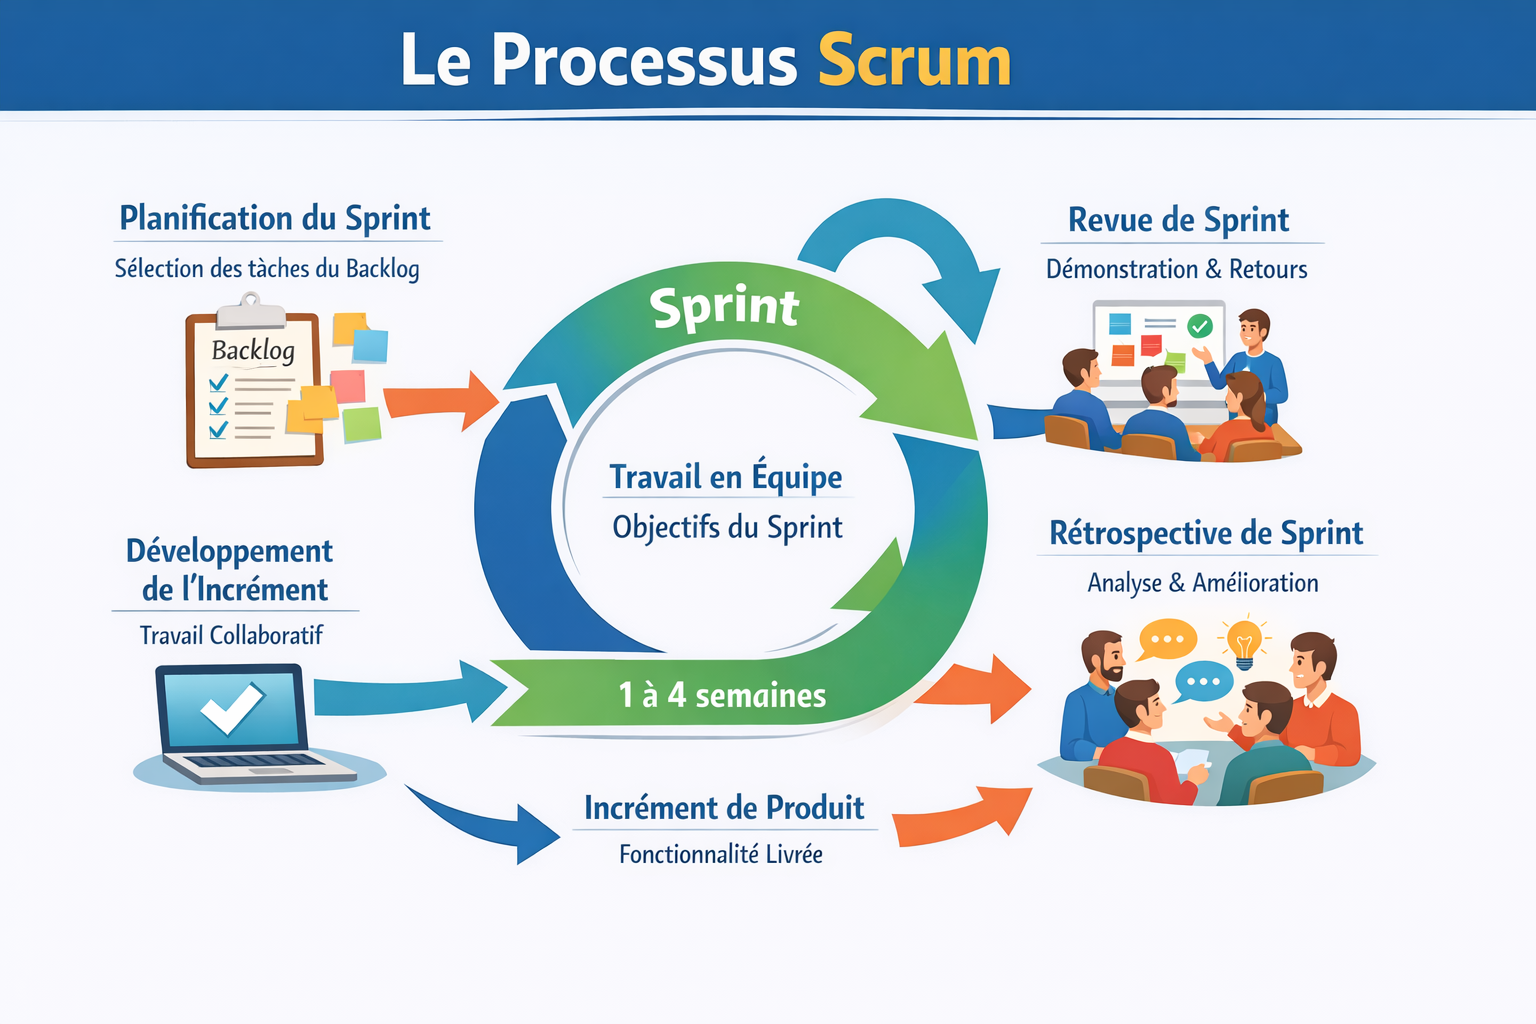
\includegraphics[width=0.9\textwidth]{scrum.png}
    \caption{Diagramme du cycle Scrum}
    \label{fig:scrum}
\end{figure}

\subsection{Raisons du choix de Scrum}
Le choix de Scrum~\cite{scrum} pour ce projet repose sur plusieurs avantages clés :
\begin{itemize}[label=\textbullet, leftmargin=1.5cm]
    \item \textbf{Livraison continue et incréments testables :} Chaque sprint produit un incrément fonctionnel et vérifiable, réduisant le risque de livrer un produit non conforme aux attentes.
    \item \textbf{Flexibilité :} Scrum permet d'intégrer facilement les changements et les nouvelles exigences tout au long du projet, sans perturber l'avancement global.
    \item \textbf{Transparence :} Les cérémonies régulières (revue, rétrospective, daily stand-up) assurent une visibilité claire sur l'état du projet et favorisent une communication fluide entre les parties prenantes.
    \item \textbf{Satisfaction client :} L'approche itérative et centrée sur la valeur métier garantit la livraison rapide de fonctionnalités utiles et adaptées aux besoins réels des clients.
    \item \textbf{Engagement de l'équipe :} Scrum encourage la collaboration, l'auto-organisation et l'amélioration continue, renforçant la motivation et l'implication des membres de l'équipe.
\end{itemize}

\subsection{Les rôles Scrum}
\begin{itemize}[label=\textbullet, leftmargin=1.5cm]
    \item \textbf{Product Owner (PO) :}
    Responsable de maximiser la valeur du produit, il gère le backlog produit, définit les priorités selon la valeur métier et communique les besoins des parties prenantes à l'équipe de développement.

    \item \textbf{Scrum Master (SM) :}
    Garant de l'application de Scrum, il facilite les cérémonies, supprime les obstacles rencontrés par l'équipe et accompagne celle-ci dans l'amélioration continue de ses pratiques.

    \item \textbf{Équipe de développement :}
    Composée de professionnels multidisciplinaires, elle est auto-organisée et responsable de la réalisation des incréments de produit à chaque sprint. L'équipe décide collectivement de la meilleure manière de transformer les éléments du backlog en fonctionnalités livrables.
\end{itemize}

\section{Langage de modélisation UML}\label{sec:uml}

Dans le cadre de la formalisation et du développement de nos idées, UML (Unified Modeling Language) constitue un langage de modélisation graphique standardisé par l'Object Management Group~\cite{uml}. Il permet de structurer, représenter et documenter un système logiciel de manière indépendante du langage de programmation utilisé. UML est également un outil de communication efficace entre les acteurs techniques et métier, offrant une représentation claire de la structure statique et du comportement dynamique des systèmes à travers différents types de diagrammes.

\begin{itemize}[label=\textbullet, leftmargin=1.5cm]
    \item \textbf{Diagramme de cas d'utilisation :}
    Le diagramme de cas d'utilisation illustre les interactions entre les acteurs et le système. Il identifie les utilisateurs (acteurs) et les fonctionnalités accessibles (cas d'utilisation). Les relations include et extend permettent de gérer les comportements communs ou optionnels. Ce diagramme constitue généralement le premier livrable dans l'analyse fonctionnelle, définissant le périmètre du système.

    \item \textbf{Diagramme de classes :}
    Le diagramme de classes représente la structure statique d'un système. Il décrit les classes, leurs attributs, leurs méthodes ainsi que les relations qui les unissent (associations, héritage, composition, agrégation). Ce diagramme sert souvent de référence pour la conception de la base de données et pour guider la génération du code.

    \item \textbf{Diagramme de séquence :}
    Le diagramme de séquence décrit la dynamique des interactions entre les composants du système dans le temps. Il montre l'ordre chronologique des messages échangés entre acteurs, objets et services pour réaliser un scénario donné. Ce diagramme est particulièrement utile pour modéliser des flux complexes incluant conditions, boucles et appels à des services externes.
\end{itemize}

\begin{figure}[htbp]
    \centering
    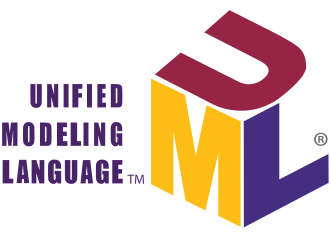
\includegraphics[width=0.5\textwidth]{UML_logo.png}
    \caption{Langage de modélisation UML}
    \label{fig:uml}
\end{figure}

\section*{Conclusion}
Ce chapitre a présenté le contexte du projet, analysé les limites des solutions existantes et justifié les choix méthodologiques adoptés. Ces éléments constituent le cadre de référence sur lequel s'appuie l'ensemble du travail de conception et de développement présenté dans les chapitres suivants.
